% -*- coding: utf-8

\documentclass[slideopt,A4]{beamer}

\usetheme{default}

\useoutertheme{infolines}

\usepackage[]{fontspec}
\usepackage{fontenc}
\usepackage[type1]{libertine}
\renewcommand{\ttdefault}{cmtt}

\usepackage{lastpage}
\usepackage{mdframed}
\usepackage[usenames,dvipsnames,svgnames,table]{xcolor}


\usepackage{eurosym}
\usepackage{url}
\usepackage{anyfontsize}
\setmainfont{linuxbiolinumo}
\setsansfont{linuxbiolinumo}

\definecolor{fontmaincolor}{HTML}{000000}
\definecolor{bgcolor}{HTML}{FFFFFF}
\definecolor{bgshadecolor}{HTML}{DDDDDD}
\graphicspath{%
  {./Figures/}%
}
%\usepackage [T1] {inputenc}
%\usepackage [utf8] {inputenc}

\usepackage{tikz}
\usetikzlibrary{arrows,patterns,plotmarks,shapes,snakes,er,3d,automata,backgrounds,topaths,trees,petri,mindmap}
\usepackage{pgfplots}
\usepackage{pgfplotstable}

\usepackage{eso-pic}
\usepackage{monster2e}
\usepackage{tikz}
\usepackage{layout}
\usepackage{xcolor}
\usepackage{amsmath,amssymb,wasysym}
\usepackage{fancybox}
\usepackage{graphicx}
\usepackage{multimedia}
\usepackage[absolute,showboxes,overlay]{textpos}
\TPshowboxesfalse
\textblockorigin{0mm}{0mm}

\usepackage{media9}
%\usepackage{movie15_dvipdfmx}
%\usepackage[dvipdfmx]{movie15_dvipdfmx}

\definecolor{rouge1}{RGB}{226,0,38}  % red P
\definecolor{orange1}{RGB}{243,154,38}  % orange P
\definecolor{jaune}{RGB}{254,205,27}  % jaune P
\definecolor{blanc}{RGB}{255,255,255} % blanc P

\definecolor{rouge2}{RGB}{230,68,57}  % red S
\definecolor{orange2}{RGB}{236,117,40}  % orange S
\definecolor{taupe}{RGB}{134,113,127} % taupe S
\definecolor{gris}{RGB}{91,94,111} % gris S
\definecolor{bleu1}{RGB}{38,109,131} % bleu S
\definecolor{bleu2}{RGB}{28,70,114} % bleu S
\definecolor{vert1}{RGB}{133,146,66} % vert S
\definecolor{vert2}{RGB}{157,193,7} % vert S

\definecolor{rouge3}{RGB}{255,200,130}  

\setbeamertemplate{navigation symbols}{}
\setbeamertemplate{blocks}[rounded][shadow=false]
\setbeamercolor{block title}{fg=white, bg=rouge1}
\setbeamercolor{block body}{fg=black, bg=rouge3}

\usepackage{tikz}
% tikz library (frise lncmi exemple)
\usetikzlibrary{calc,fit,shadows,arrows,positioning}
\usepackage{xcolor}
\xdefinecolor{fColor}{RGB}{0 81 145} % Light blue
\newcommand{\fColor}{fColor}

\newcommand{\topLegend}[2]{
  node [text centered,%
  shade,%
  top color=\fColor,%
  text justified,
  draw,%
  semithick,
  rounded corners=2pt,
  above,
  #1] {#2}}

\newcommand{\bottomLegend}[2]{
  node [text centered,%
  shade,%
  top color=\fColor,%
  text justified,
  draw,%
  semithick,
  rounded corners=2pt,
  below,
  #1] {#2}}

\newcommand{\topEvent}[3]{\draw[<-,very thick] (#1) coordinate (#2) (#2 |- xH axis) -- ++ (#3)}
\newcommand{\bottomEvent}[3]{\draw[<-,very thick] (#1) coordinate (#2) -- ++ (#3)}
\newcommand{\bottomGraphics}[2]{node[below,draw,inner sep=1pt,thin,rounded corners=1pt] {\includegraphics[#1]{#2}}}
\newcommand{\topGraphics}[2]{node[above,draw,inner sep=1pt,thin,rounded corners=1pt] {\includegraphics[#1]{#2}}}

% define trademark symbol
\def\registered{{\ooalign{\hfil\raise .00ex\hbox{\scriptsize R}\hfil\crcr\mathhexbox20D}}}

\renewcommand{\sfdefault}{lmss}
\sffamily

\setbeamersize{text margin left=1cm,text margin right=1cm}


\AtBeginSection[] {
  \begin{frame}<beamer>{Plan}
   \tableofcontents[sectionstyle=show/shaded,subsectionstyle=show/shaded/hide]
%    \tableofcontents[currentsection]
  \end{frame}
 }

\AtBeginSubsection[] {
  \begin{frame}<beamer>{Plan}
   \tableofcontents[sectionstyle=show/shaded,subsectionstyle=show/shaded/hide]
%    \tableofcontents[currentsection,currentssubection]
  \end{frame}
 }


\newcommand{\ds}{\displaystyle}
\newcommand{\dg}{^\circ}
\newcommand{\saut}{\vspace*{3mm}\\}
\newcommand{\RR}{\hbox{\bf I\hspace*{-1mm}R}}
%% Macros
\newcommand{\ddx}[1]{\ensuremath{\frac{\partial #1}{\partial x}}}
\newcommand{\ddy}[1]{\ensuremath{\frac{\partial #1}{\partial y}}}
\newcommand{\ddz}[1]{\ensuremath{\frac{\partial #1}{\partial z}}}
\newcommand{\dddxdx}[1]{\ensuremath{\frac{\partial^2 #1}{\partial x \partial x}}}
\newcommand{\dddxdy}[1]{\ensuremath{\frac{\partial^2 #1}{\partial x \partial y}}}
\newcommand{\dddydy}[1]{\ensuremath{\frac{\partial^2 #1}{\partial y \partial y}}}
\renewcommand{\div}{\operatorname{div}}
\renewcommand{\rot}{\operatorname{rot}}

\begin{document}


\setbeamertemplate{background canvas}[vertical shading][top=white,middle=white,bottom=white]

\setbeamertemplate{footline}{ \hspace{5em} \textcolor{white} {Les Mathématiques}\hspace{2em}\null \vspace*{3pt}}


\begin{frame}

\begin{textblock*}{15cm}(13mm,30mm)
{\textcolor{red} {
{\huge\bf Mathématiques appliquées: }\\[2mm]
{\huge\bf  des maths en lien avec la société}\\[2mm]
{\bf Modélisation Simulation et Optimisation}\\[8mm] }}
{\textcolor{black} {
%   	{\Large Philippe Helluy \& Christophe Prud'homme}\\[2mm]
	{\Large Université de Strasbourg}\\[2mm]
        
\includegraphics[height=1.2cm]{LOGOS/logoCemosis}	\hspace*{40mm}	
        
\includegraphics[height=1.2cm]{LOGOS/logoUDS}\\
      }}
\end{textblock*}

\end{frame}


%%%%%%%%%%%%%%%%%%%%%%%%%%%

\setbeamertemplate{background canvas}[vertical shading][top=blanc, middle=blanc,bottom=blanc]

\setbeamercolor{toto}{fg=white,bg=blue}

\setbeamertemplate{footline}
{
\begin{beamercolorbox}[wd=1\paperwidth,ht=15.5pt]{toto}
\hspace{-1.6mm}	
  \raisebox{1.2ex}
  {  
\includegraphics[height=.6cm]{LOGOS/logoCemosis}}
  \raisebox{2.5ex}
  %{ P. Helluy \& C. Prud'homme (UNISTRA/CEMOSIS)  }
  {Cemosis, IRMA, UFR Math-Info}
\hspace{\fill}	
 % \raisebox{1.2ex}
%\hspace{\fill}	
%  \raisebox{2.5ex}
%  { \insertframenumber \hspace{1mm}  }
  \raisebox{2.5ex}
 {  }
  \raisebox{1ex}
{  \colorbox{white}{
\includegraphics[height=.6cm]{LOGOS/logoUDS}}}
\end{beamercolorbox} 
}

%
%
%%%%%%%%%%%%%%%%%%%%%%%%%%%%%%%%%%%%%%

\begin{frame}{{\Large Plan}}
  \tableofcontents
  % Vous pouvez, si vous le souhaiter ajouter l'option [pausesections]
\end{frame}



%\begin{frame}
%Crypto: ajouter exemple de codage / décodage  eco spé maths TS\\[10mm]
%
%Simul: faire la discrétisation d'une équation de transport: 
%- on prend 2 boites, on écrit les quantités qui passent de l'une à l'autre en un pas de temps delta t
%- puis on en prend 3, etc...
%
%\end{frame}

%%%%%%%%%%%

\section{Mathématiques appliquées et métiers des maths}



\begin{frame}
\frametitle{Pour commencer...}

%\textcolor{black} 
%
%
%\begin{minipage}{70mm}
\begin{itemize}
\item {\large A quoi servent les mathématiques ?}
\item  {\large Y a-t-il des métiers après des études en mathématiques ?}
\end{itemize}
%\end{minipage}
%
\begin{center}
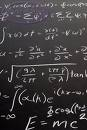
\includegraphics[width=0.20\linewidth]{maths2}$\quad$
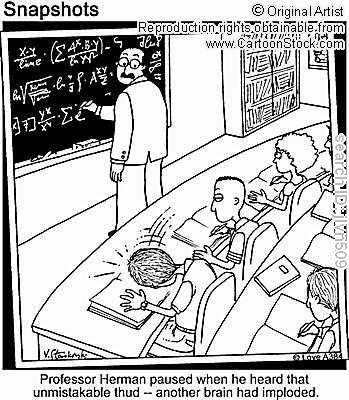
\includegraphics[width=0.27\linewidth]{maths1}$\quad$
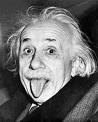
\includegraphics[width=0.24\linewidth]{einstein}
\end{center}

\begin{block}{Du coté de nos amis américains?}
  \begin{itemize}
  \item Un métier en pleine expansion: \\{\small\url{http://www.bls.gov/ooh/math/mathematicians.htm}}
  \item Best job en 2014:\\ {\small \url{http://www.careercast.com/jobs-rated/best-jobs-2014}}
  \end{itemize}
\end{block}
%
\end{frame}



%%%%%%%%%%%%%%%%%%%%%



\begin{frame}
\frametitle{Les mathématiques sont omniprésentes dans notre société}
%
%Les mathématiques sont omniprésentes dans notre société.
\begin{center}
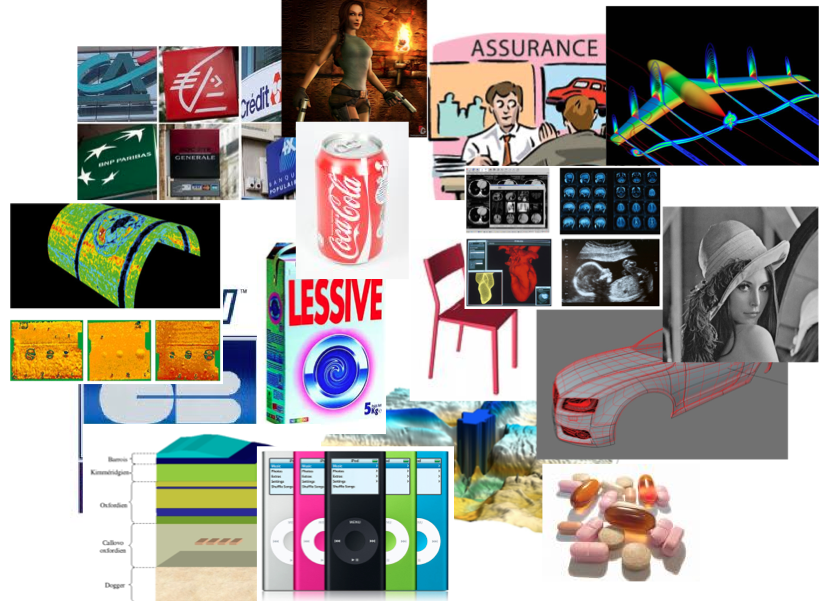
\includegraphics[width=0.90\linewidth]{mix.png}
\end{center}

\end{frame}
%
%

\begin{frame}
\frametitle{Créer des images...}
%
\begin{center}
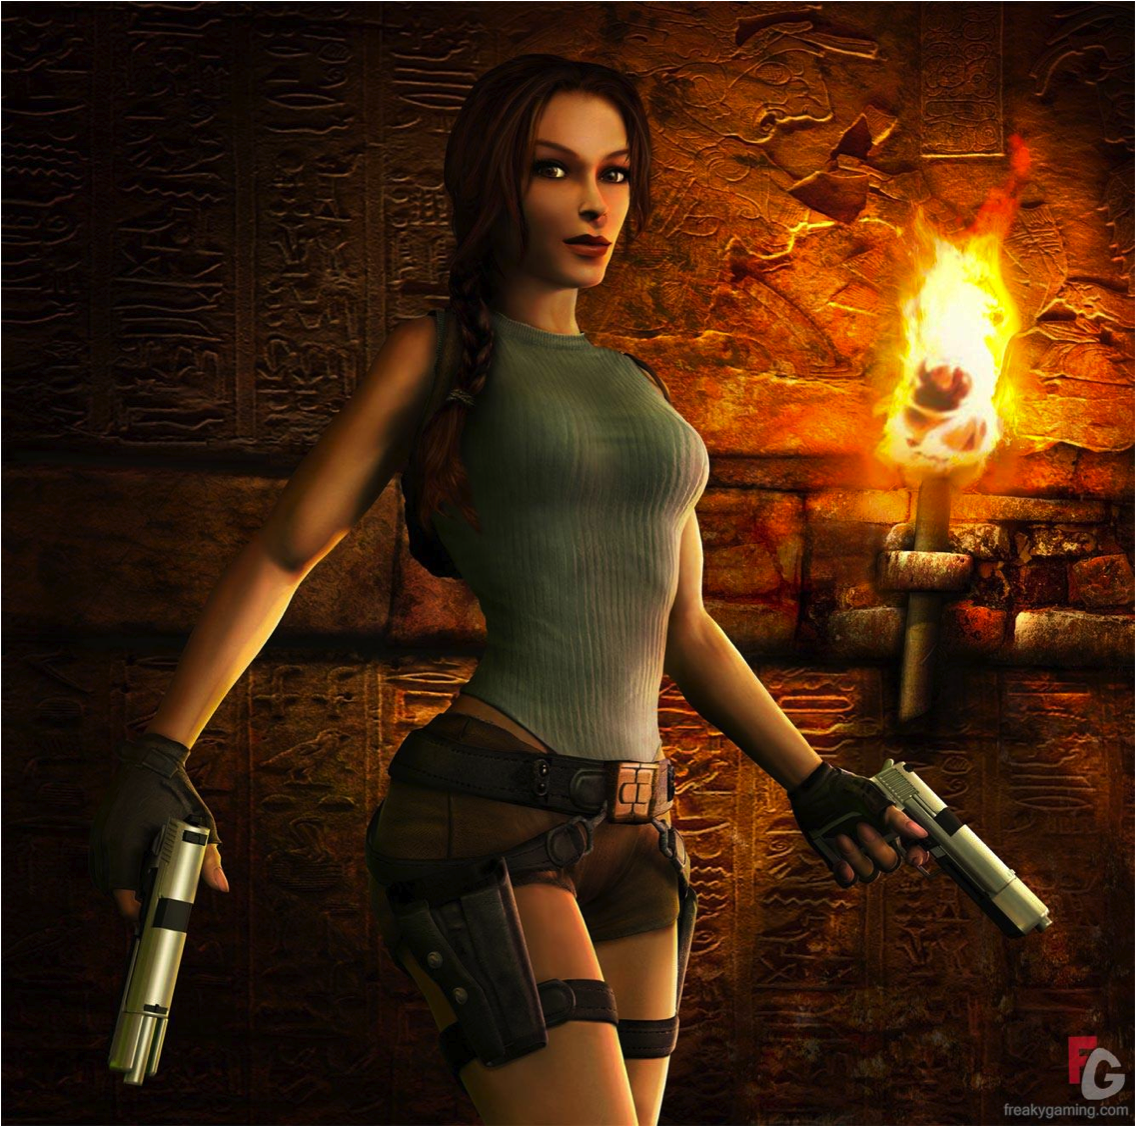
\includegraphics[width=0.40\linewidth]{LaraCroft.png}$\,$
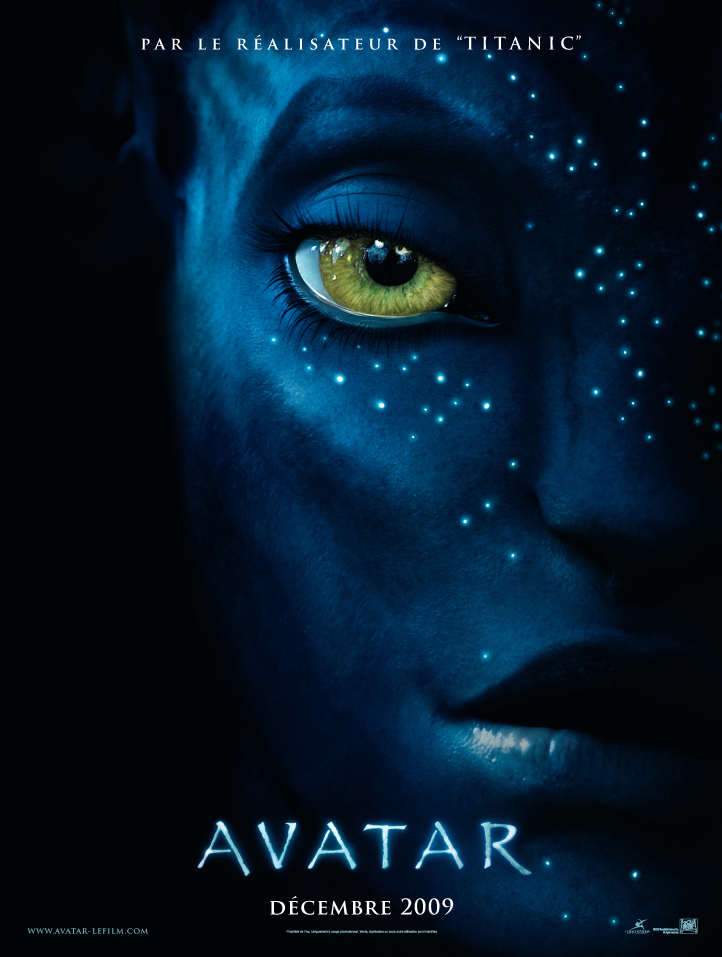
\includegraphics[width=0.30\linewidth]{avatar}\\
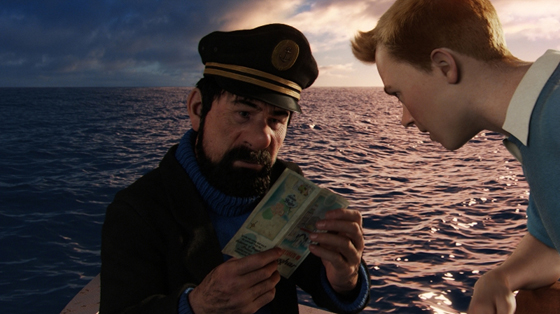
\includegraphics[width=0.50\linewidth]{tintin}
\end{center}
%
\end{frame}
%
%
\begin{frame}
\frametitle{Créer des images...}
%
\begin{center}
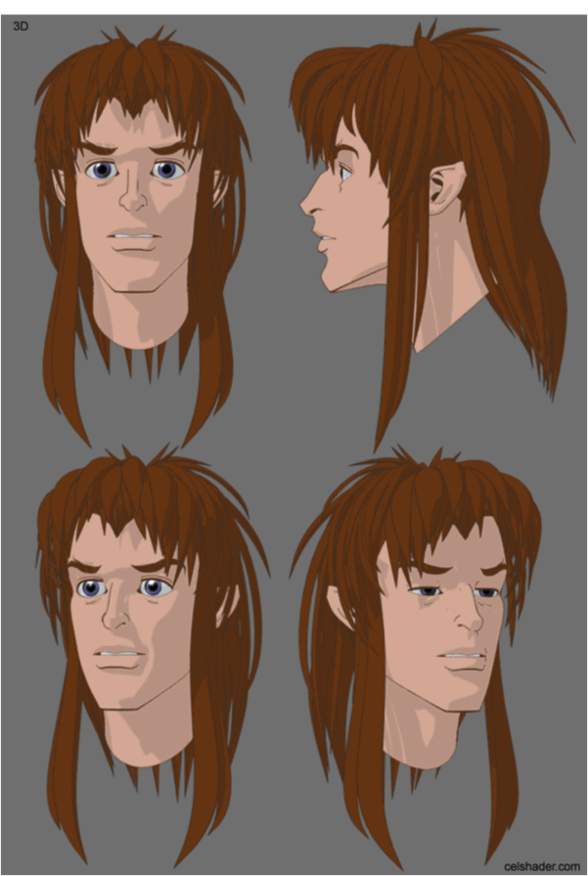
\includegraphics[width=0.40\linewidth]{tete.png}$\quad$
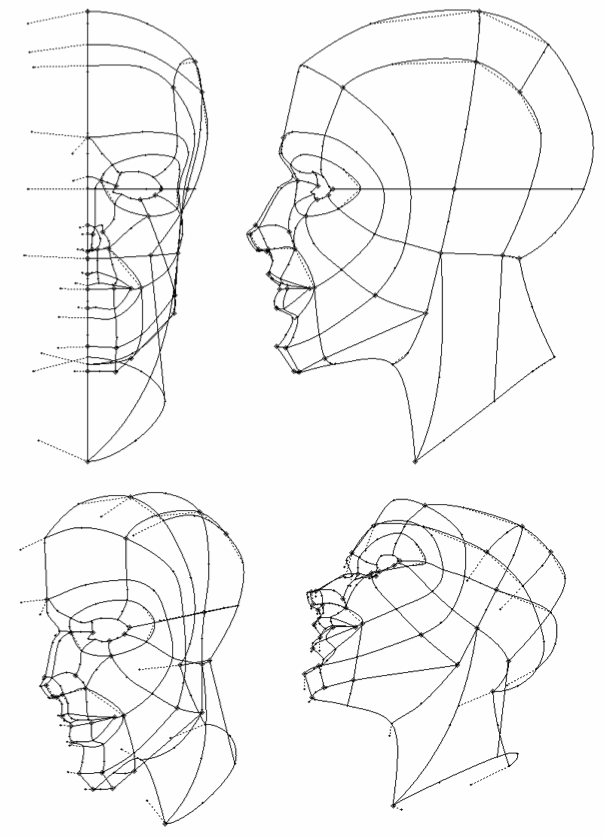
\includegraphics[width=0.40\linewidth]{tete2.png}
\end{center}
%
\end{frame}
%


%
\begin{frame}
\frametitle{Compresser les images et les sons: MP3, MP4, jpeg, mov...}
%
\begin{center}
\begin{tabular}{cc}
\textcolor{red}{Image originale} & \textcolor{red}{Image compressée} \\
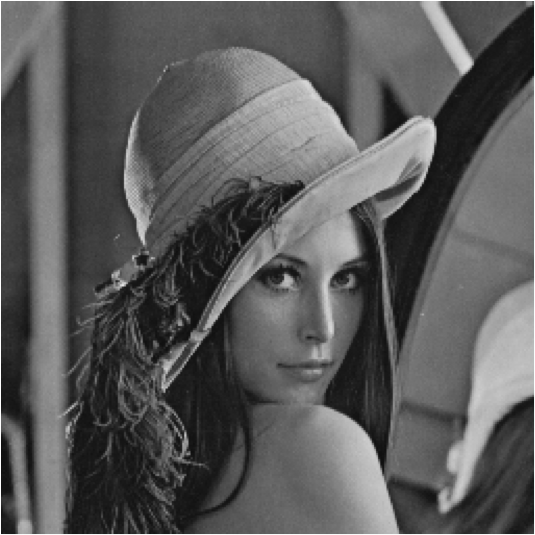
\includegraphics[width=0.40\linewidth]{lana-original.png} &
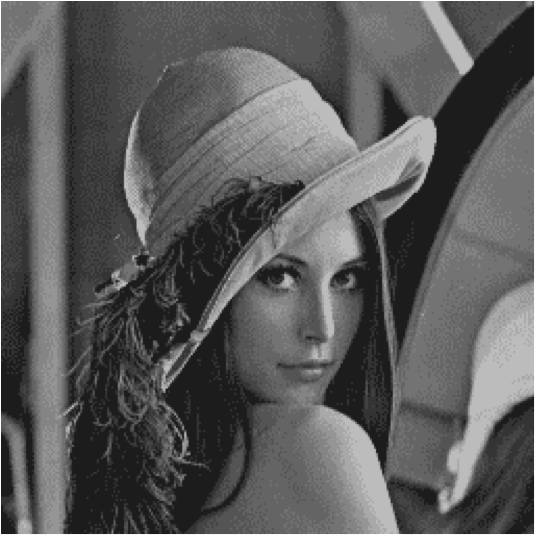
\includegraphics[width=0.40\linewidth]{lana-compresse.png}
\end{tabular}
\end{center}
%
\pause
%
\begin{center}
~\\[-10mm]
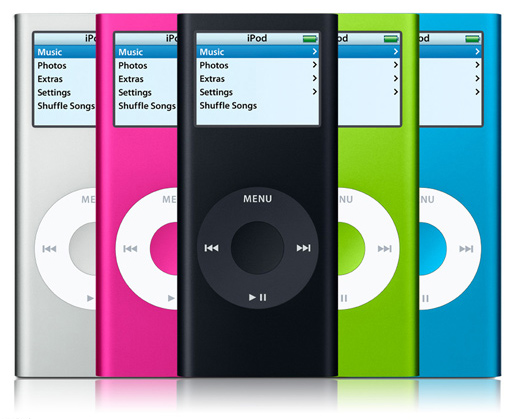
\includegraphics[width=0.4\linewidth]{ipod.jpg}
\end{center}
%
\end{frame}
%

%
\begin{frame}
\frametitle{Compresser les images et les sons: MP3, MP4, jpeg, mov...}
%
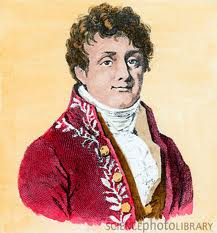
\includegraphics[width=0.3\linewidth]{fourier} $\qquad$
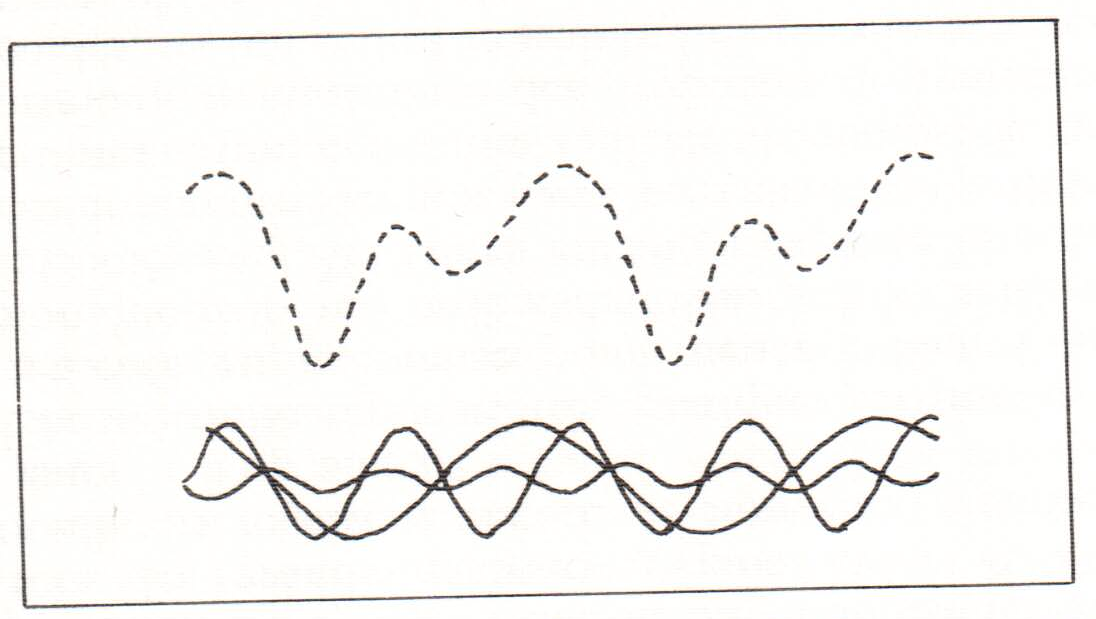
\includegraphics[width=0.5\linewidth, angle=-1.5]{fourier4} \\[5mm]
\centerline{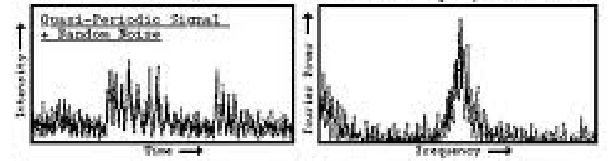
\includegraphics[width=0.6\linewidth]{fourier2}}
%
\end{frame}
%

%
\begin{frame}
\frametitle{Imagerie médicale...}
\small
%
%
\begin{block}{Principe}
On soumet le corps à un signal (magnétique, électrique, acoustique, ...), et en fonction de la réponse obtenue, on reconstruit  une image de la zone observée (problème inverse).
\end{block}
%
\centerline{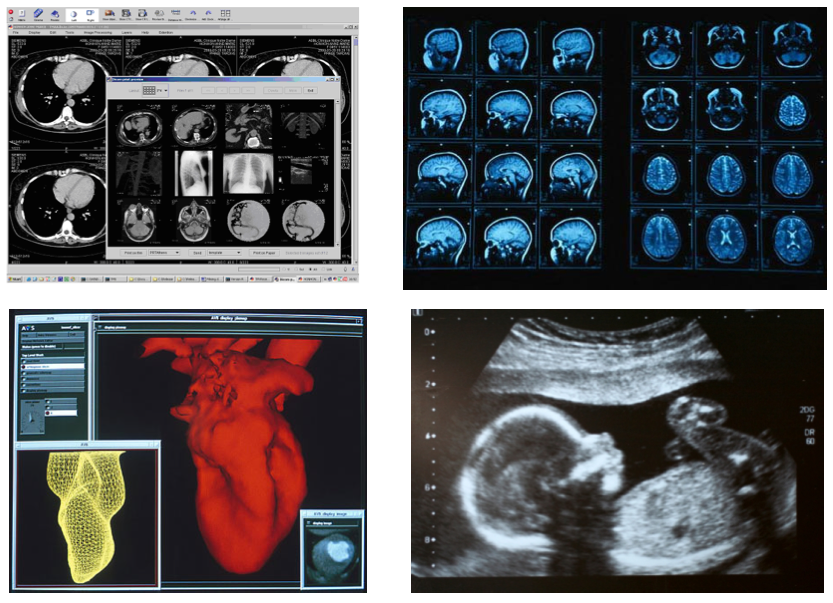
\includegraphics[width=0.7\linewidth]{imagerie-medicale.png}}
%
\end{frame}
%

\begin{frame}
  \frametitle{Santé}
  
  \begin{block}{}
    Comprendre les mécanismes physiologiques et
    pathologiques(anévrismes, anémie, atherosclérose, maladies
    neurodégénératives: Alzheimer...),
    proposer des outils de diagnostics peu chers et fiables
  \end{block}

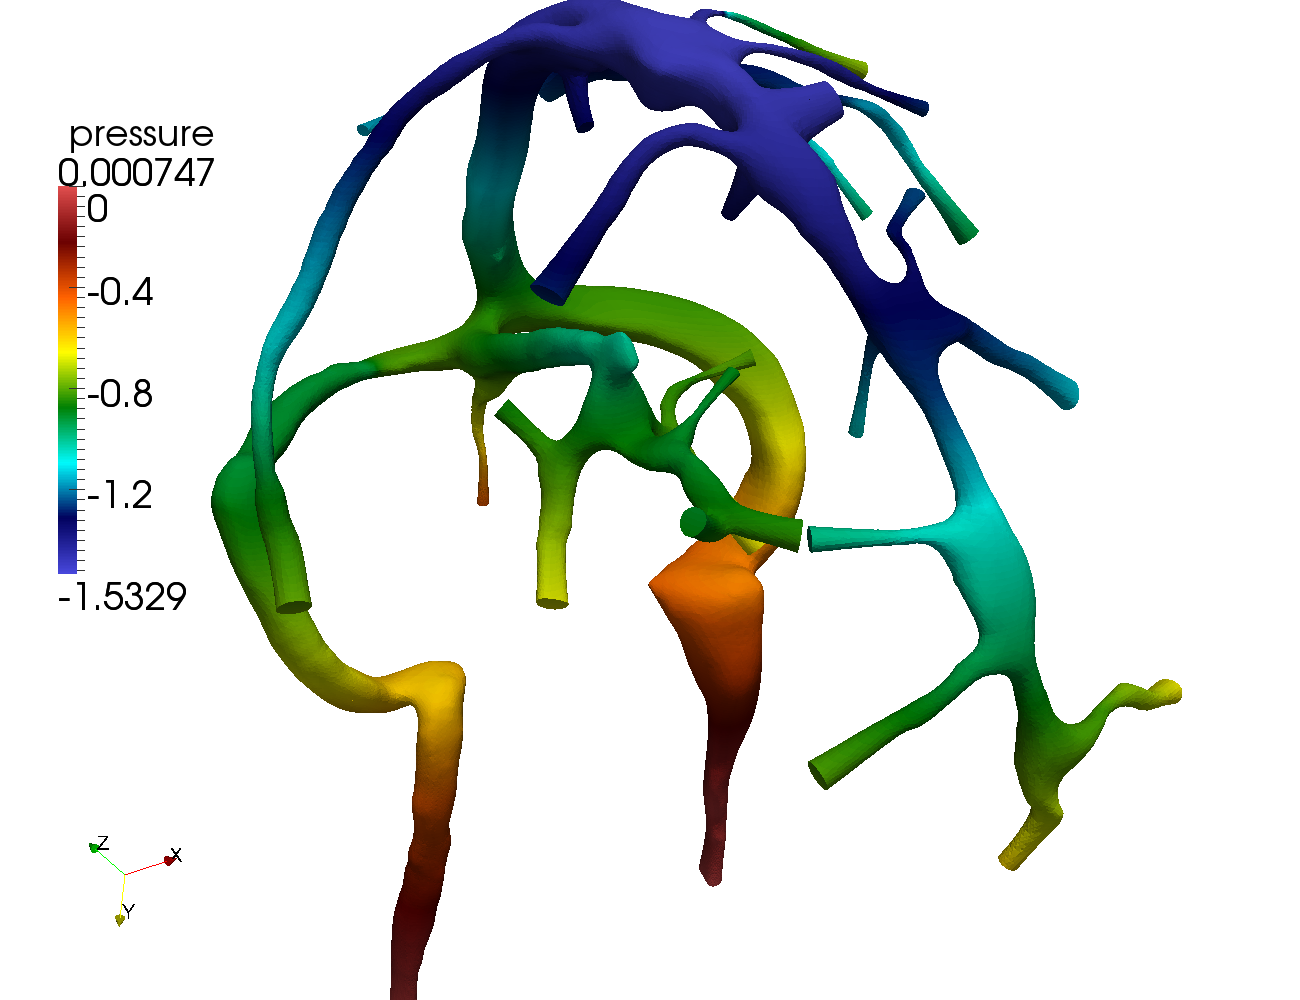
\includegraphics[width=0.3\linewidth]{Figures/MesoChallengePressure2.png}$\;$
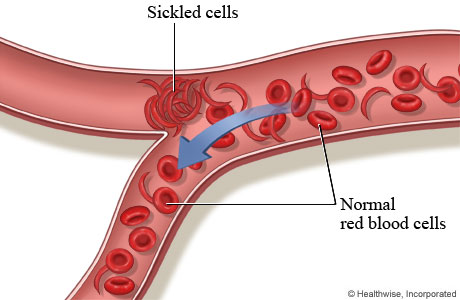
\includegraphics[width=0.3\linewidth]{Figures/sickleCellDisease.jpg}$\;$
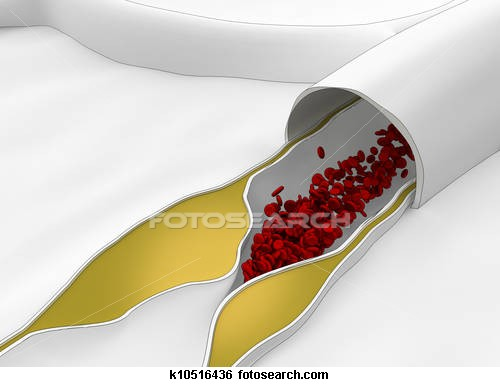
\includegraphics[width=0.3\linewidth]{Figures/atherosclerosisDisease.jpg}\\
\centerline{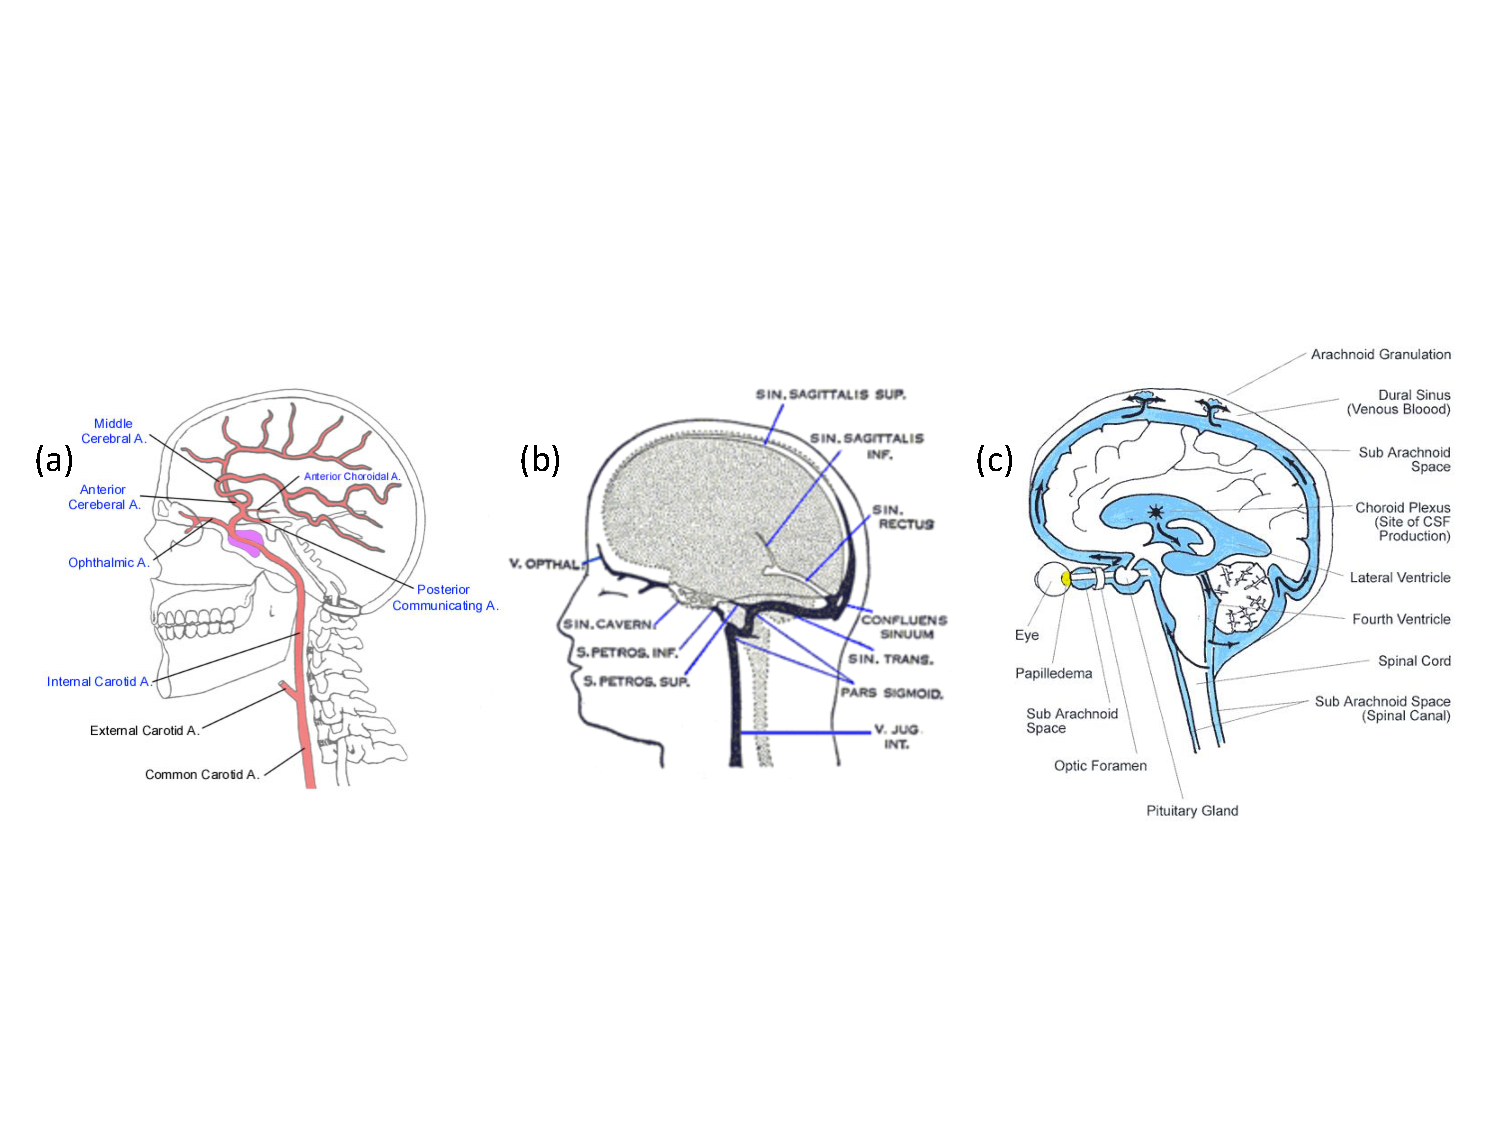
\includegraphics[width=0.6\linewidth]{Figures/Eye2Brain_connections.pdf}}
  
\end{frame}
%
\begin{frame}
\frametitle{Statistiques...}
%
%
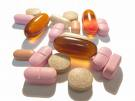
\includegraphics[width=0.3\linewidth]{medicaments.jpg}$\;$
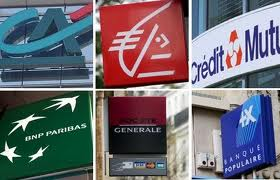
\includegraphics[width=0.3\linewidth]{banque}$\;$
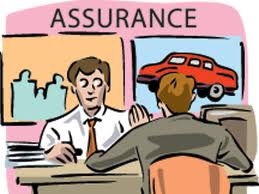
\includegraphics[width=0.3\linewidth]{assurance}
%
\end{frame}
%


%
\begin{frame}
\frametitle{Crypter...}
%
% 
\begin{minipage}{5cm}
~\\[-50mm]
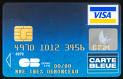
\includegraphics[width=0.75\linewidth]{carte-bleue.jpg}\\
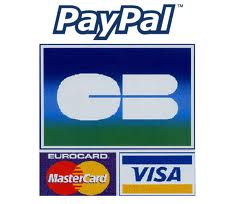
\includegraphics[width=0.95\linewidth]{paypal.jpg}
\end{minipage}
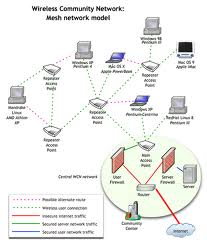
\includegraphics[width=0.5\linewidth]{reseau}
%
\end{frame}
%

\begin{frame}{Sécurité informatique : application de la théorie des nombres}

 \begin{center}
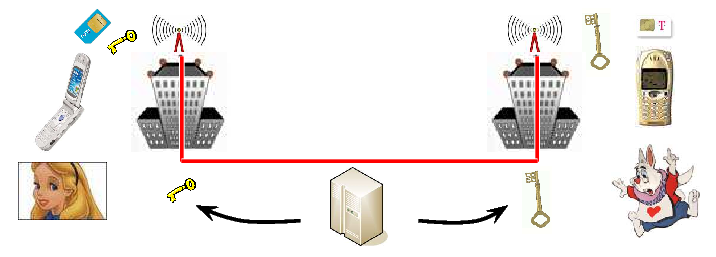
\includegraphics[scale=.45]{Sim-mobile}\\ 
 \end{center}

 SIM(Subscriber Identity Module) contient les clefs secrétes pour
 l'authentification des t\'el\'ephones, et les clefs de sessions pour
 les communications. Principe des clefs publiques / privées.  \vfill
\end{frame}

%
\begin{frame}
\frametitle{Modéliser...}
%
%
\begin{minipage}{35mm}
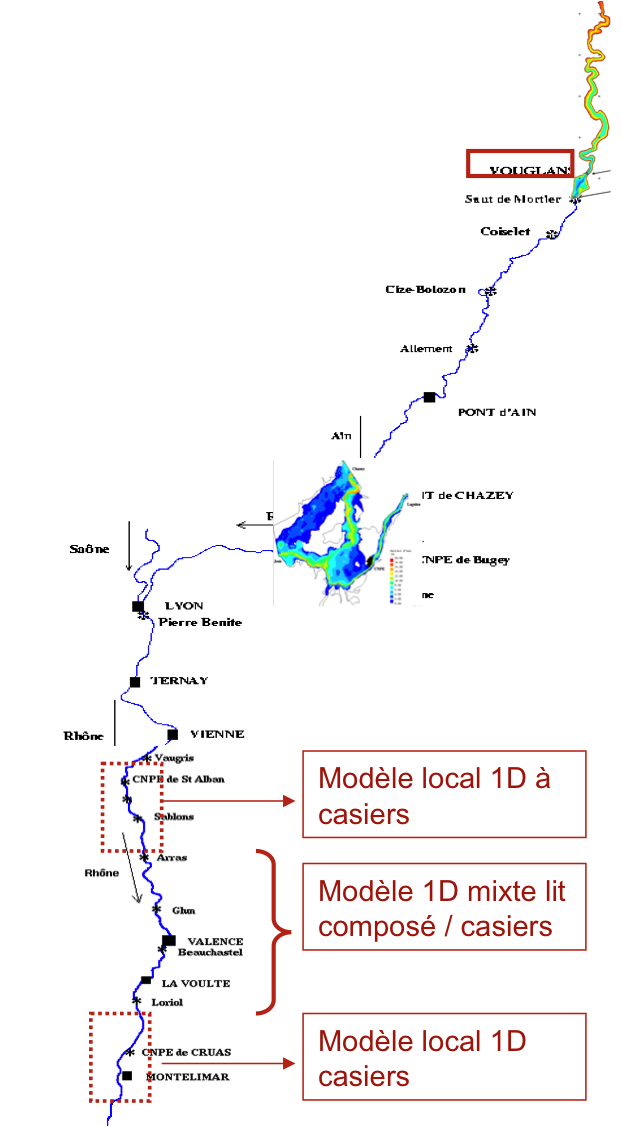
\includegraphics[width=0.99\linewidth]{edf.png}
\end{minipage}$\;$
\begin{minipage}{70mm}
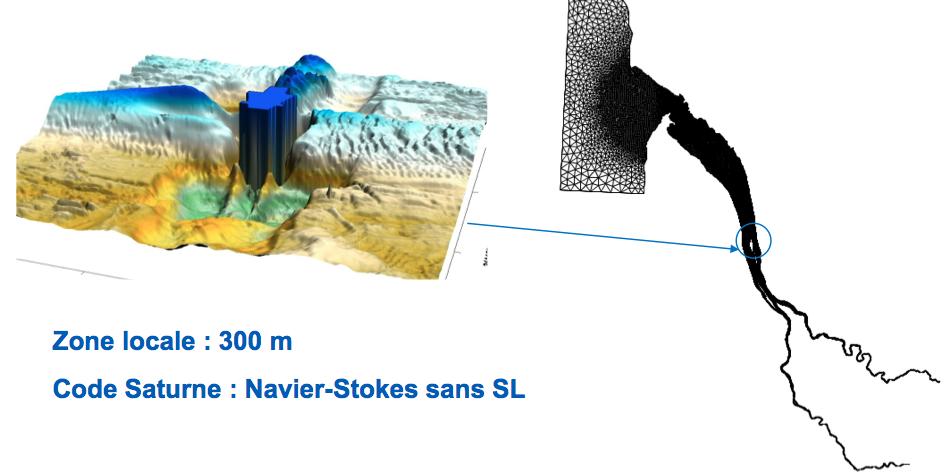
\includegraphics[width=0.99\linewidth]{edf2.png}\\[10mm]
\centerline{\alert{EDF}}
\end{minipage}
%
\end{frame}
%

%
\begin{frame}
\frametitle{Modéliser...}
%
Stockage de déchets radioactifs $\rightarrow$ Modélisation des écoulements en milieux poreux autour du site\\
\centerline{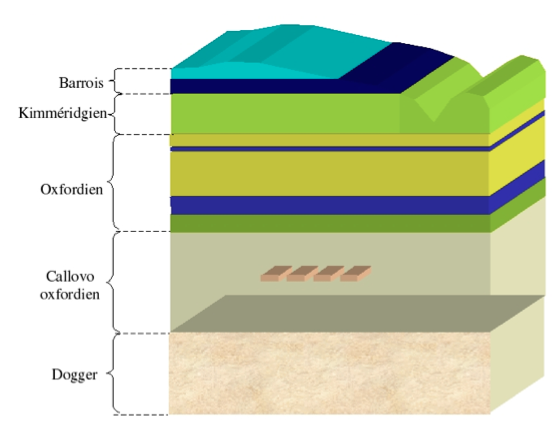
\includegraphics[width=0.8\linewidth]{stockage.png}}
%
\end{frame}
%

%
\begin{frame}
\frametitle{Modéliser...}
%
Contrôle non destructif
%
\centerline{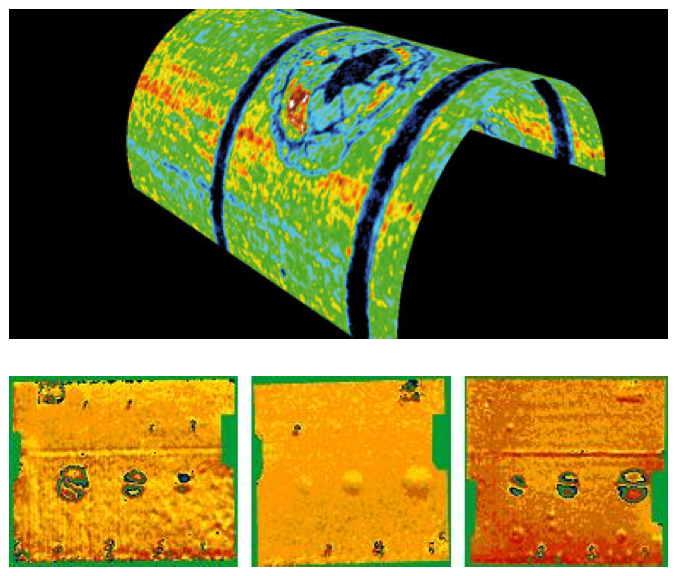
\includegraphics[width=0.75\linewidth]{controle-nondestructif.png}}
%
\end{frame}
%


%
\begin{frame}
\frametitle{Modéliser...}
%
Fusion nucléaire contrôlée : plasma confiné dans la chambre magnétique (ITER)
%
\centerline{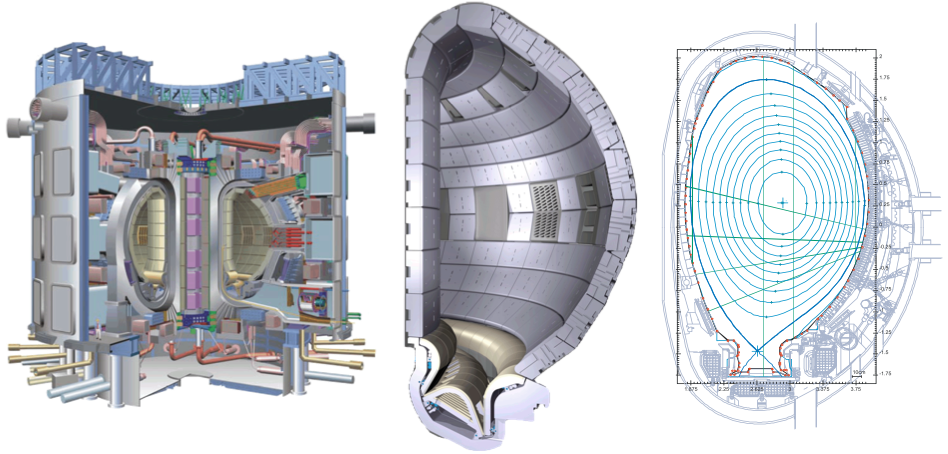
\includegraphics[width=0.8\linewidth]{iter.png}}
%
\end{frame}
%




%
\begin{frame}
\frametitle{Modéliser...}
%
% 

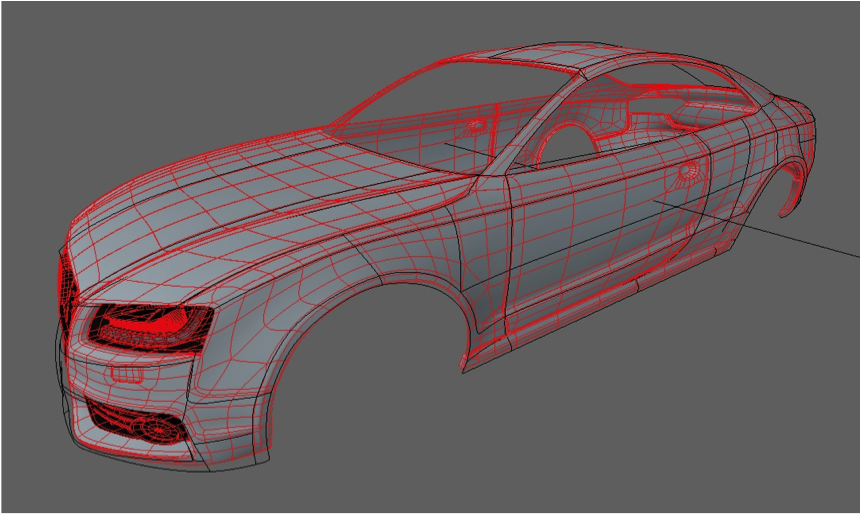
\includegraphics[width=0.4\linewidth]{voiture.png}$\qquad$
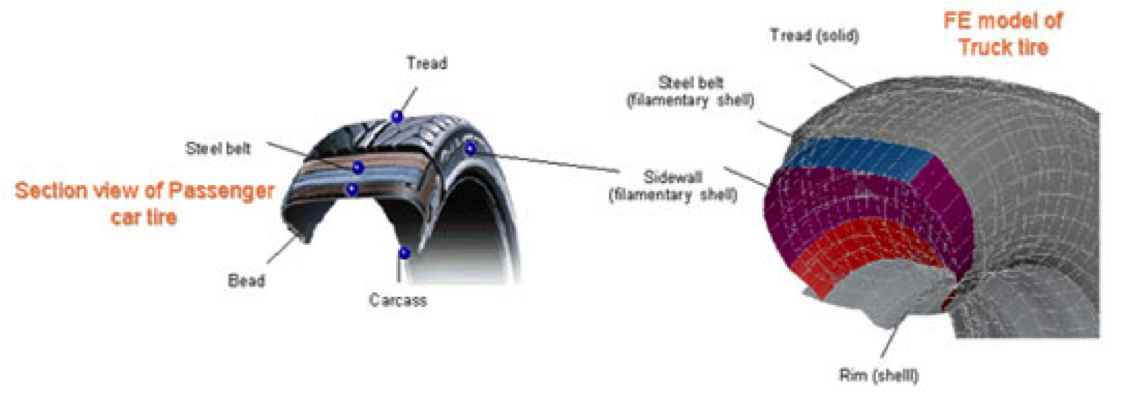
\includegraphics[width=0.5\linewidth]{pneu.png}\\[3mm]
\centerline{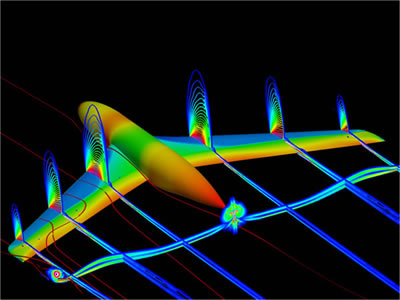
\includegraphics[width=0.5\linewidth]{avion}}
%
\end{frame}
%

%
\begin{frame}
\frametitle{Modéliser...}
%
% 
\centerline{
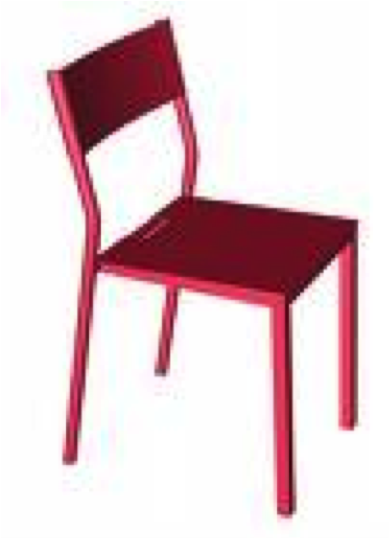
\includegraphics[width=0.2\linewidth]{chaise.png}$\qquad$
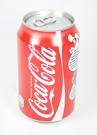
\includegraphics[width=0.2\linewidth]{coca}$\qquad$
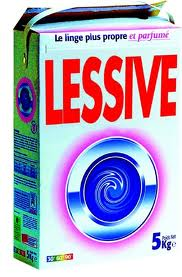
\includegraphics[width=0.2\linewidth]{lessive} }
%
\end{frame}
%
\begin{frame}
  \frametitle{Calculer...}
  TGCC Curie: 10080 eight-core processors, Intel® Xeon® Next
  Generation, un total de 80640 cores.
  \centerline{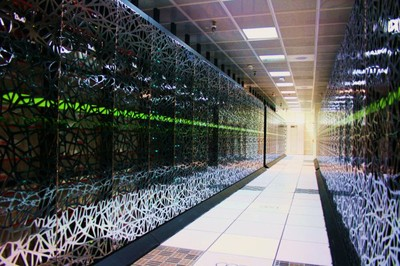
\includegraphics[width=0.8\linewidth]{Figures/tgcc_curie.jpeg}}
\end{frame}

%
\begin{frame}
\frametitle{Il y a des dizaines de "métiers des maths" {\small (pas seulement prof !) }}
%
\begin{center}
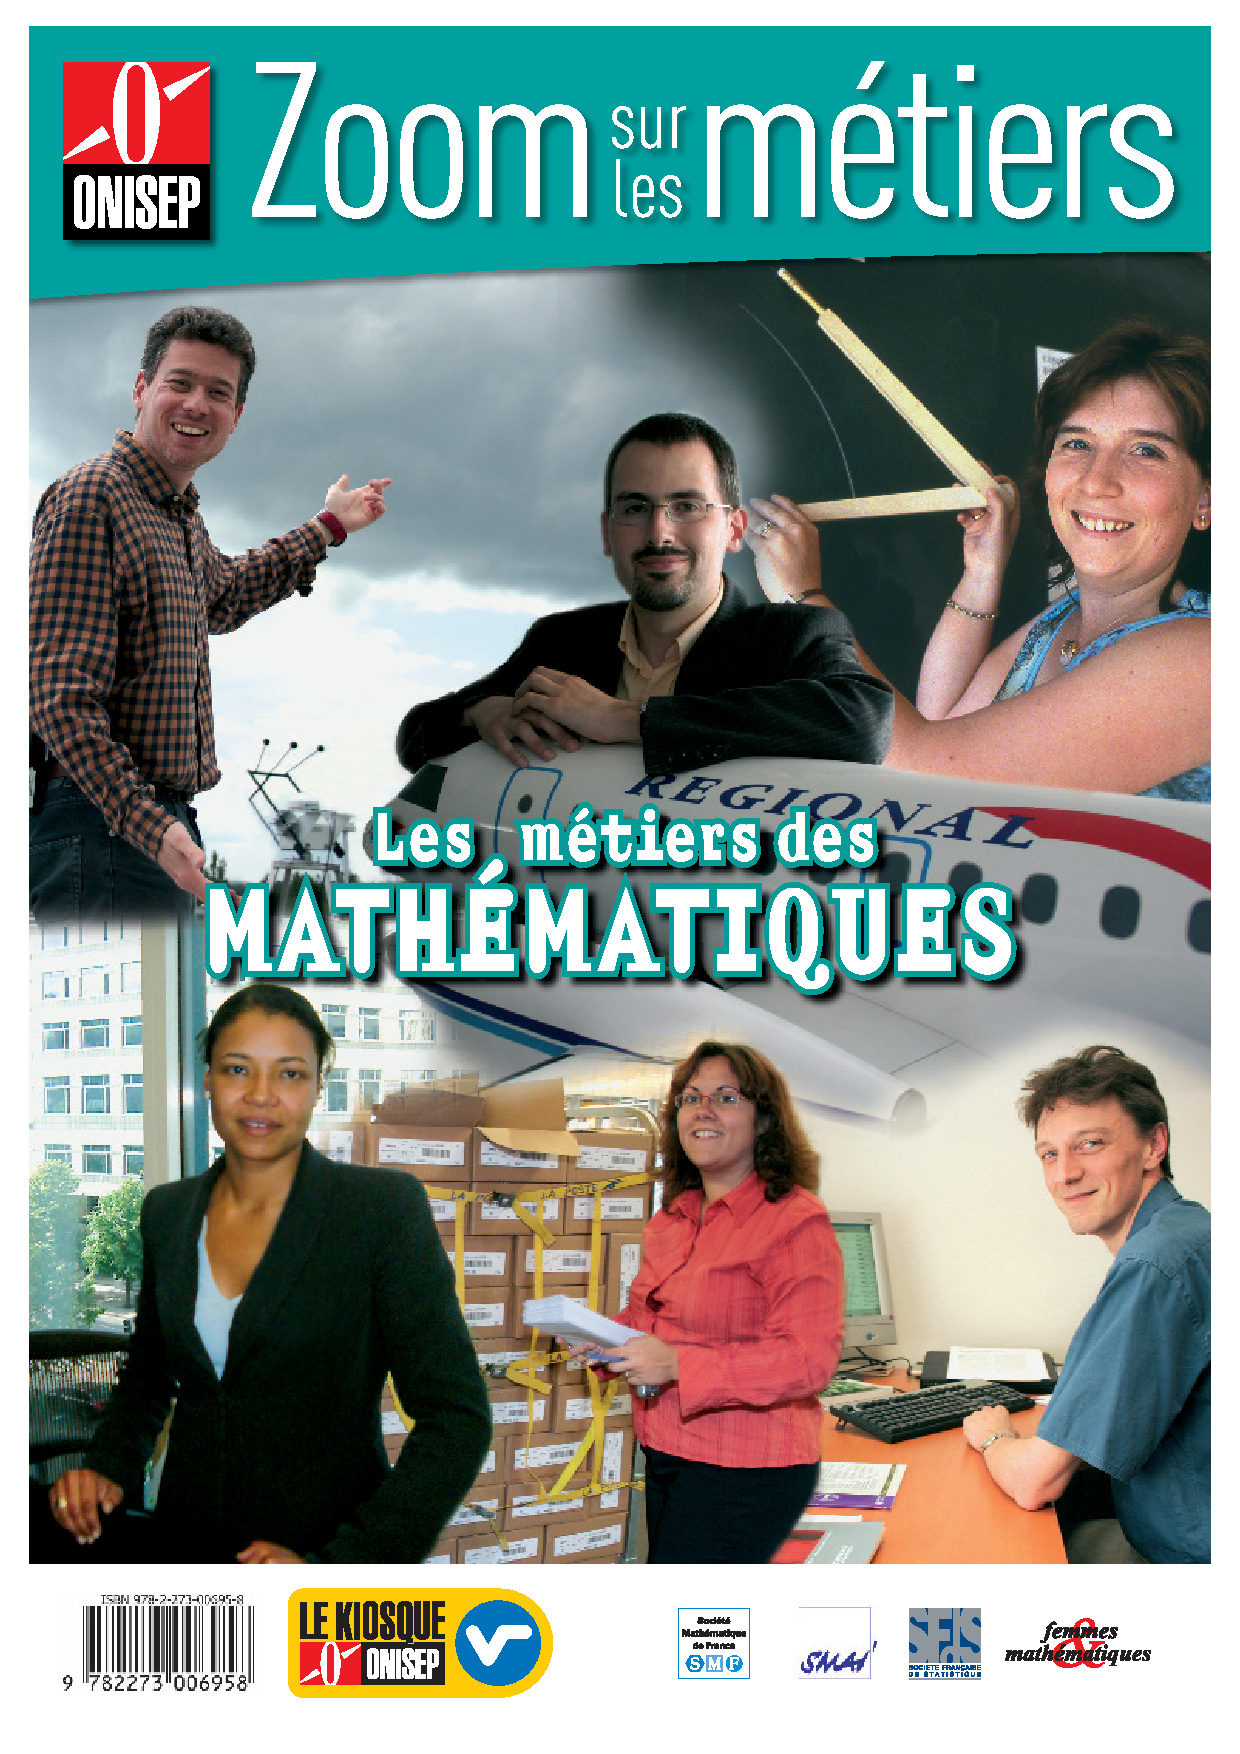
\includegraphics[width=0.4\linewidth]{onisep.pdf}
\end{center}
%
\centerline{\htmladdnormallink{Quels Métiers pour les matheux? (ONISEP!)}{http://www.onisep.fr/Toute-l-actualite-nationale/Decouvrir-les-metiers/Decembre-2014/Quels-metiers-pour-les-matheux}}
%
\end{frame}

\section{Formations et Débouchés}
% ou Comment parvenir à travailler sur  ces sujets}




\begin{frame}
  \frametitle{Les Formations de Master à Strasbourg}
  \begin{block}{Master mention Mathématiques et Applications}
    \begin{itemize}
    \item \htmladdnormallink{Spécialité Calcul Scientifique et Mathématiques de
      l'Information (CSMI)}{http://mathinfo.unistra.fr/offre-de-formation/master-mention-mathematiques-et-applications/csmi/}
    \item \htmladdnormallink{Spécialité Mathématiques Fondamentales, parcours Recherche}{http://mathinfo.unistra.fr/offre-de-formation/master-mention-mathematiques-et-applications/maths-fondamentales-recherche/}
    \item \htmladdnormallink{Spécialité Mathématiques Fondamentales, parcours Magistère de Mathématiques}{http://mathinfo.unistra.fr/offre-de-formation/master-mention-mathematiques-et-applications/maths-fondamentales-magistere/}
    \item \htmladdnormallink{Spécialité Statistique, parcours Biostatistique et Statistiques Industrielles}{http://mathinfo.unistra.fr/offre-de-formation/master-mention-mathematiques-et-applications/statistique-bio-indus/}
    \item \htmladdnormallink{Spécialité Statistique, parcours Actuariat}{http://mathinfo.unistra.fr/offre-de-formation/master-mention-mathematiques-et-applications/statistique-actuariat/}
    \item \htmladdnormallink{Agrégation}{http://mathinfo.unistra.fr/offre-de-formation/master-mention-mathematiques-et-applications/master-agregation/}
    \item \htmladdnormallink{CAPES}{http://mathinfo.unistra.fr/offre-de-formation/master-mention-mathematiques-et-applications/capes/}
    \end{itemize}  
  \end{block}
\end{frame}

\begin{frame}
  \frametitle{CSMI}
  \begin{block}{Un master pour qui ?}
    Le Master est fait pour les étudiants de Licence désirant faire
    \begin{itemize}
    \item une carrière d'ingénieur
    \item une carrière de chercheur
    \item une carrière d'enseignant-chercheur
    \end{itemize}
  \end{block}
  
  
  \begin{block}{Objectif}
  Double compétence en Calcul Scientifique et Mathématiques de l'information
  \end{block}

\end{frame}

\begin{frame}
  \frametitle{Pré-requis CSMI}
  \begin{block}{}
    Bonnes bases en analyse, en algèbre et en informatique. 
    Goût pour la programmation, l'algorithmique et les applications des mathématiques.
  \end{block}
  \centerline{Un parcours en Licence menant à CSMI}
  \begin{columns}[t]
    \column{.3\linewidth}
    \begin{block}{L1}
      
    \end{block}
    \column{.3\linewidth}
    \begin{block}{L2}
      
    \end{block}
    \column{.3\linewidth}
    \begin{block}{L3}
      
    \end{block}
  \end{columns}

\end{frame}
%%% Local Variables: 
%%% mode: latex
%%% TeX-master: "slides-math-formations-metiers"
%%% End: 


\section{Conclusion}

\begin{frame}{Les Mathématiques au coeur de la Modélisation, la Simulation et l'Optimisation}
  
\begin{itemize}
\item Un travail très pluri-disciplinaire  (le matheux n'est pas seul)
\item Des maths, souvent récentes, sont sous-jacentes un peu partout (même si on ne les voit pas)
\item De nombreux défis (mathématiques) pour les années à venir %: couplage de modèles, quantification des incertitudes ...
\end{itemize}


\end{frame}






\end{document}

